%%%%%%%%%%%%%%%%%%%%%%%%%%%%%%%%%%%%%%%%%%%%%%%%%%%%%%%%%%%%%%%%%%%%%%%%%%%%%%%%
% Template for USENIX papers.
%
% History:
%
% - TEMPLATE for Usenix papers, specifically to meet requirements of
%   USENIX '05. originally a template for producing IEEE-format
%   articles using LaTeX. written by Matthew Ward, CS Department,
%   Worcester Polytechnic Institute. adapted by David Beazley for his
%   excellent SWIG paper in Proceedings, Tcl 96. turned into a
%   smartass generic template by De Clarke, with thanks to both the
%   above pioneers. Use at your own risk. Complaints to /dev/null.
%   Make it two column with no page numbering, default is 10 point.
%
% - Munged by Fred Douglis <douglis@research.att.com> 10/97 to
%   separate the .sty file from the LaTeX source template, so that
%   people can more easily include the .sty file into an existing
%   document. Also changed to more closely follow the style guidelines
%   as represented by the Word sample file.
%
% - Note that since 2010, USENIX does not require endnotes. If you
%   want foot of page notes, don't include the endnotes package in the
%   usepackage command, below.
% - This version uses the latex2e styles, not the very ancient 2.09
%   stuff.
%
% - Updated July 2018: Text block size changed from 6.5" to 7"
%
% - Updated Dec 2018 for ATC'19:
%
%   * Revised text to pass HotCRP's auto-formatting check, with
%     hotcrp.settings.submission_form.body_font_size=10pt, and
%     hotcrp.settings.submission_form.line_height=12pt
%
%   * Switched from \endnote-s to \footnote-s to match Usenix's policy.
%
%   * \section* => \begin{abstract} ... \end{abstract}
%
%   * Make template self-contained in terms of bibtex entires, to allow
%     this file to be compiled. (And changing refs style to 'plain'.)
%
%   * Make template self-contained in terms of figures, to
%     allow this file to be compiled. 
%
%   * Added packages for hyperref, embedding fonts, and improving
%     appearance.
%   
%   * Removed outdated text.
%
%%%%%%%%%%%%%%%%%%%%%%%%%%%%%%%%%%%%%%%%%%%%%%%%%%%%%%%%%%%%%%%%%%%%%%%%%%%%%%%%

\documentclass[letterpaper,twocolumn,10pt]{article}
\usepackage{usenix2019_v3}

% to be able to draw some self-contained figs
\usepackage{tikz}
\usepackage{amsmath}

% inlined bib file
\usepackage{filecontents}

\usepackage{graphicx}
\graphicspath{{\downloads }}

%-------------------------------------------------------------------------------
\begin{filecontents}{\jobname.bib}
%-------------------------------------------------------------------------------
@Book{arpachiDusseau18:osbook,
  author =       {Arpaci-Dusseau, Remzi H. and Arpaci-Dusseau Andrea C.},
  title =        {Operating Systems: Three Easy Pieces},
  publisher =    {Arpaci-Dusseau Books, LLC},
  year =         2015,
  edition =      {1.00},
  note =         {\url{http://pages.cs.wisc.edu/~remzi/OSTEP/}}
}
@InProceedings{waldspurger02,
  author =       {Waldspurger, Carl A.},
  title =        {Memory resource management in {VMware ESX} server},
  booktitle =    {USENIX Symposium on Operating System Design and
                  Implementation (OSDI)},
  year =         2002,
  pages =        {181--194},
  note =         {\url{https://www.usenix.org/legacy/event/osdi02/tech/waldspurger/waldspurger.pdf}}}
\end{filecontents}

%-------------------------------------------------------------------------------
\begin{document}
%-------------------------------------------------------------------------------
% make title bold and 14 pt font (Latex default is non-bold, 16 pt)
\title{\Large \bf CS 131: Homework 3 Report}
\author{Java shared memory performance races}
\maketitle

%-------------------------------------------------------------------------------
\section{Introduction}
%-------------------------------------------------------------------------------

This report will discuss the results gathered by running a modified Java program under a given test harness using two different servers - lnxsrv06 and lnxsrv11. In addition, I will explore topics mentioned in Lea's paper, such as data race conditions and how they relate to VarHandle methods and operations. 



%-------------------------------------------------------------------------------
\section{AcmeSafeState implementation}
%-------------------------------------------------------------------------------
By using the java.util.concurrent.atomic.AtomicLongArray object, I was able to surpass the performance of SynchronizedState (exact figures will be shown later on in the report). Since part of the challenge was to avoid using locks / mutexes, I used a form of atomic increments and decrements to achieve the desired behavior. Namely, the 
void swap(int i, int j) method within my implementation of AcmeSafeState utilized two functions from the java.until.concurrent.atomic package getAndIncrement(i) and getAndDecrement(i). The memory effects of these functions,as specified by  VarHandle.getAndAdd(java.lang.Object...) VarHandle references are rather dynamic - as Lea states, "they can be associated with any field, array element, or static, allowing control over access modes." 

%-------------------------------------------------------------------------------
\section{Data Race Free?}

In the implementation of UnsynchronizedState, which intentionally disallows the use of locks and the "synchronized" keyword, threads are accessing, reading, and writing to memory concurrently. Data races are bountiful here, as threads are allowed to break sequential consistency. This causes particularly nasty behavior - namely a "sum mismatch" within this particular program. My implementation for AcmeSafeState is free of data races, as it performs atomic operations which eschew issues related to schedulers and thread interference / conflicts. 

%-------------------------------------------------------------------------------

\section{Problems Faced}

Although I didn't run into too many problems when designing my program, I ran into
a few issues when testing on the various servers. It was a bit tedious gathering results for every benchmark, so I used an Excel spreadsheet to help me keep track of my data. Instead of dumping the data directly into this report, I created a few bar graphs to maximize user readability.

\begin{figure}
\caption{Error Message}
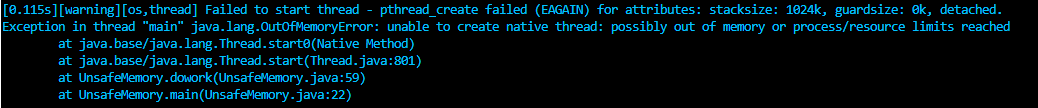
\includegraphics[scale=.25, width=0.9\columnwidth]{limitsreached.PNG}
\end{figure}

I received the error message depicted in Figure 1 when attempting to run the test harness with a thread count of 40 on lnxsrv06. Any thread count above 35-36 proved to be impossible to run, as the memory/resource capacities were at their limit on this particular virtual machine. As I do not have a local machine to test these on, I simply omitted the results for these specific test cases per the advice of my TA. I've included the results from lnxsrv11, however. To overcome this problem, I simply capped the number of threads at 35 when testing - this also served as the thread count of "my choice" as specified in the project spec.

%--------------------------

\section{Measurements and Results}
\subsection{lnxsrv06}
\begin{figure}
\caption{}
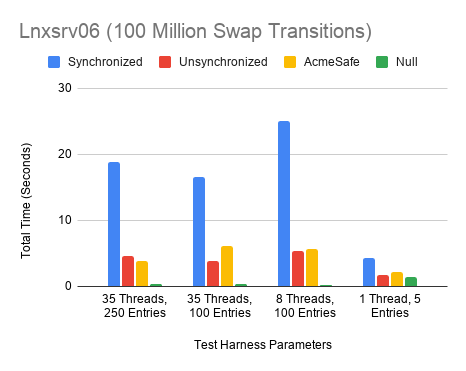
\includegraphics[scale=.5]{lnxsrv06.png} 
 \end{figure}
 


As shown in Figure 2, the total time to complete the required operations with 0 sum mismatches was \textbf{significantly} higher when running the SynchronizedState class. The program took upwards of 25 seconds to complete when running 8 threads and only 100 entries - curious, since the test that was ran with 35 threads and 100 entries performed nearly 10 seconds faster. Of course, the tests ran with the baseline Null program took less than a second, as expected. It appears as if the AcmeSafeState class performed quite well, especially when compared even to the Unsynchronized speeds. AcmeSafe ran slightly slower than Unsynchronized in all but one category, where it slightly outperformed when ran with 35 threads and using a state array of 250 entries. As mentioned earlier, no tests with 40 threads were ran for this server, due to server capacity limits. 
\\

A general trend that can be observed is that more threads leads to increased time: likely due to increased overhead required for the swap transitions (with the exception of the test that required 8 threads). In general, AcmeSafe performed faster than Synchronized consistently - this is good news, as it is preventing data races while still minimizing overhead required with locking functions in Synchronized. While Unsynchronized is faster overall, it is a practically broken program that allows sequential consistency violations. GDI will not want anything to do with such an implementation.
\\


\subsection{lnxsrv11} 
\begin {figure}
\caption{}
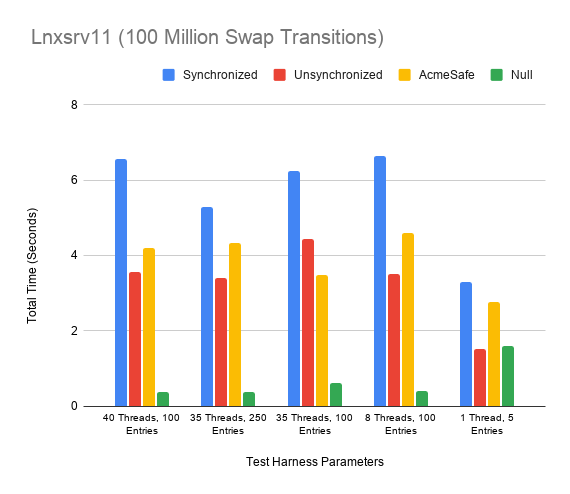
\includegraphics[scale=.45]{lnxsrv11.png}  
\end{figure}

lnxsrv11 fared much better in terms of overall performance: no test ran for more than 8 seconds. This is likely do to it being severely less overwhelmed, resource-wise, when compared to lnxsrv06. As expected, Null state runs in less than a second for all but one of the tests done - our baseline program appears to be working. Just as in the tests ran on lnxsrv06, Synchronized performed much worse than both Unsynchronized and AcmeSafe (Figure 3). AcmeSafe performed only marginally worse than Unsynchronized for each test, except where it outperformed Unsynchronized when ran with 35 threads and 100 entries. Since I was able to run the test harness with more 35 threads on this server, I have included those results in this chart as well. AcmeSafe fared relatively well, ans it performed only slower than Unsynchronized which was just a few ns shy of 4 seconds. As noted in the analysis of the results from lnxsrv06, the less threads ran, typically the faster the output(again, curiously with the exception of 8 threads). Again, AcmeSafe still appears to be more efficient than Synchronized, as its atomic operations are less costly while still preventing thread contention. 
%-----------------------------------

\section{Final Thoughts}
Overall, it seems as if AcmeSafe is the winner of these brief experiments. Again, it consistently outperforms Synchronized across servers by a large gap, and is only slightly slower than Unsynchronized. Thanks to Lea's documentation, it was easy to get a grasp on why this is the case and why locks can be so expensive to a program. It also became clear on how certain flaws in the Java Memory Model can lead to severe security-breaking consequences through means of data race side effects such as pointer forgery. Regardless, GDI should see through the implementation of AcmeSafeState due to its consistently strong performance and DRF compliance. 


\section*{Acknowledgments}
%-------------------------------------------------------------------------------

Much appreciation to Chi Zhang and the other TAs for their assistance with this assignment, as well as Professor Eggert.

%-------------------------------------------------------------------------------

%-------------------------------------------------------------------------------
\bibliographystyle{plain}
\bibliography{\jobname}
\section* {References}
gee.cs.oswego.edu/dl/html/j9mm.html
\\ 
https://web.cs.ucla.edu/classes/winter21/cs131/hw/hw3.html
%%%%%%%%%%%%%%%%%%%%%%%%%%%%%%%%%%%%%%%%%%%%%%%%%%%%%%%%%%%%%%%%%%%%%%%%%%%%%%%%
\end{document}
%%%%%%%%%%%%%%%%%%%%%%%%%%%%%%%%%%%%%%%%%%%%%%%%%%%%%%%%%%%%%%%%%%%%%%%%%%%%%%%%

%%  LocalWords:  endnotes includegraphics fread ptr nobj noindent
%%  LocalWords:  pdflatex acks
